% vim: spell
\documentclass[11pt,oneside,draft]{fithesis2}

%\usepackage[draft]{pgf}
\usepackage{tikz}

%\usepackage[slovak]{babel}
\usepackage[english]{babel}
\usepackage[utf8]{inputenc}
\usepackage[T1]{fontenc}
\usepackage[plainpages=false,pdfpagelabels,unicode]{hyperref}

\usepackage{lmodern}
\usepackage{amsmath,amsthm,amsfonts}
%\usepackage{ae}

\usepackage{fancyvrb}
\usepackage{enumerate}
\clubpenalty=1000
\widowpenalty=1000
\renewcommand{\baselinestretch}{1.08}

%% Symbols used in generated graphics
%\newcommand{\kindStar}{\star}
\newcommand{\kindStar}{{\star}}
\newcommand{\hasType}{~{:}~}
\newcommand{\hasKind}{\,{:}\,}
\newcommand{\typeTo}{\mathrel{\mathop{\to}}}
\newcommand{\kindTo}{\mathrel{\mathop{\to}}}
\newcommand{\typeDot}{\,.\,}
\newcommand{\inj}{\hookrightarrow}


\DefineVerbatimEnvironment{code}{Verbatim}
        { fontsize=\small
        , commentchar=@
        , frame=single
        %, numbers=left
        %, framesep=5pt
        %, fontshape=sl
        , commandchars=\\\{\}
        , framesep=5pt
        %, fontshape=sl
        }

\newtheorem{lemma}{Lemma}
\newtheorem{example}{Example}

%\thesistitle{Rozšírenia typového systému pre Haskell}
\thesistitle{Extensions of Haskell type system}
%\thesissubtitle{Diplomová práca}
%\thesissubtitle{Master Thesis}
\thesissubtitle{Diploma Thesis}
\thesisstudent{Matej Kollár}
\thesiswoman{false}
\thesisfaculty{fi}
%\thesisyear{jar 2011}
\thesisyear{autumn 2011}
\thesisadvisor{Libor Škarvada, RNDr.}
%\thesislang{sk}
\thesislang{en}

\begin{document}
\FrontMatter
\ThesisTitlePage

\begin{ThesisDeclaration}
\DeclarationText
\AdvisorName
\end{ThesisDeclaration}

\begin{ThesisThanks}
I would like to thank to Libor, Zuzana and mommy.
\end{ThesisThanks}

\begin{ThesisAbstract}
The aim of the master's thesis/work is to provide...
\end{ThesisAbstract}

% XXX! Check whether they are relevant.
\begin{ThesisKeyWords}
Haskell, type system, type extension
\end{ThesisKeyWords}

\tableofcontents

\MainMatter

\chapter{Introduction}

\chapter{Type system}

% XXX: Move this to introduction?
Talking about extensions of type system requires understanding what type system is.
In this work we will understand type system (similarly as
\cite{pierce:2002:types,barendregt:1992:lambdaProc}) a formal system providing

\begin{description}
	\item[safety] -- meaningless or invalid code can be detected at compile time,
	\item[optimization] -- useful information might be obtained as a by-product of static type-checking,
	\item[documentation] -- types provide information on how various parts can be combined together,
	\item[abstraction] -- types provided higher level of thinking about programs,
	\item[specification] -- specifying type narrows possibilities how to write down programs,
		eliminating many wrong-ones.
\end{description}

Static typing, Strong typing, \dots

\section{Haskell type system}

Before discussing extensions it would be desirable to describe
original type system itself.
As one can find not only in \cite{haskell2010}, Haskell uses a traditional
Hindley-Milner polymorphic type system to provide a static type
semantics enriched with type classes that provide structural way to
introduce overloaded functions.

\noindent
\begin{figure}
	\centering
	\scalebox{0.9}{ 
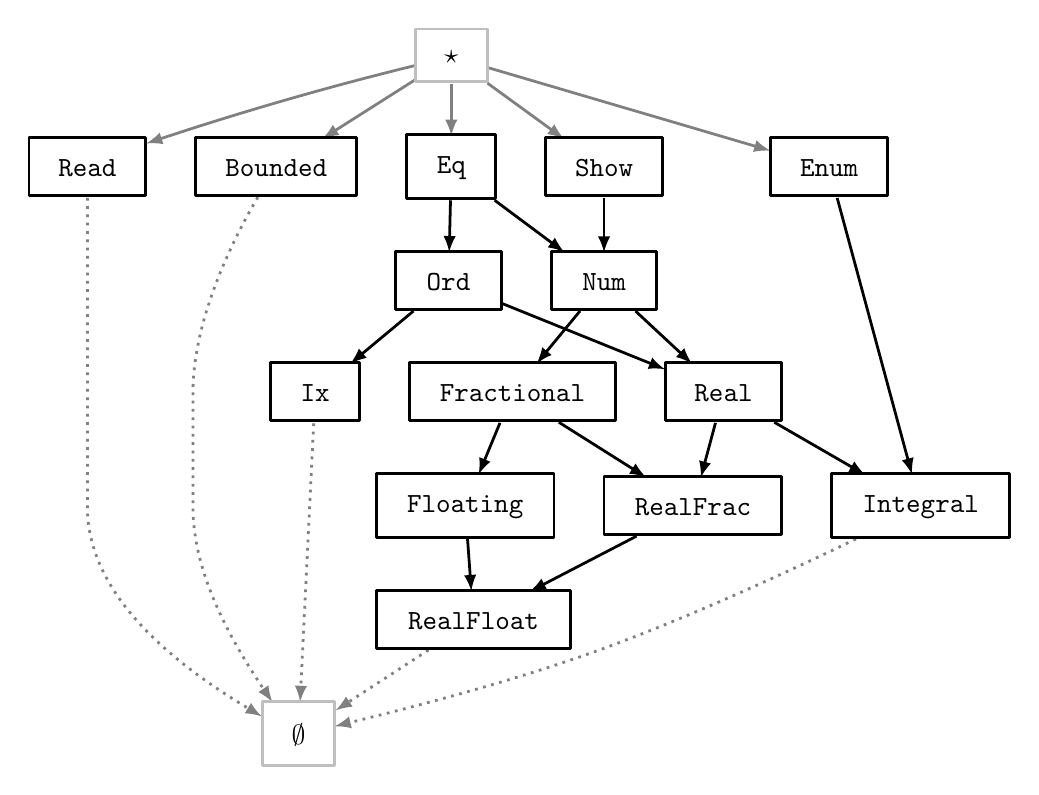
\begin{tikzpicture}[>=latex,line join=bevel,]
  \pgfsetlinewidth{1bp}
%%
\pgfsetcolor{black}
  % Edge: \texttt{Eq} -> \texttt{Num}
  \draw [->] (167.61bp,204.36bp) .. controls (172.91bp,200.42bp) and (178.92bp,195.93bp)  .. (192.67bp,185.69bp);
  % Edge: \texttt{Show} -> \texttt{Num}
  \draw [->] (207bp,205.23bp) .. controls (207bp,202.29bp) and (207bp,199bp)  .. (207bp,185.56bp);
  % Edge: \kindStar -> \texttt{Read}
  \pgfsetcolor{gray}
  \draw [->] (138.79bp,252.83bp) .. controls (120.95bp,248.45bp) and (88.037bp,240.01bp)  .. (42.198bp,224.81bp);
  % Edge: \kindStar -> \texttt{Enum}
  \draw [->] (165.04bp,252.16bp) .. controls (186.09bp,245.97bp) and (228.14bp,233.61bp)  .. (266.82bp,222.23bp);
  % Edge: \texttt{Ix} -> \emptyset
  \draw [->,dotted] (102.47bp,124.08bp) .. controls (101.48bp,103.92bp) and (99.364bp,60.469bp)  .. (97.575bp,23.787bp);
  % Edge: \kindStar -> \texttt{Show}
  \draw [->] (165.03bp,246.52bp) .. controls (170.71bp,242.39bp) and (177.54bp,237.42bp)  .. (192.51bp,226.54bp);
  % Edge: \texttt{Floating} -> \texttt{RealFloat}
  \pgfsetcolor{black}
  \draw [->] (157.85bp,82.361bp) .. controls (158.05bp,79.7bp) and (158.26bp,76.793bp)  .. (159.22bp,63.685bp);
  % Edge: \texttt{RealFloat} -> \emptyset
  \pgfsetcolor{gray}
  \draw [->,dotted] (143.78bp,42.441bp) .. controls (136.17bp,37.493bp) and (127bp,31.525bp)  .. (110.41bp,20.725bp);
  % Edge: \texttt{Fractional} -> \texttt{Floating}
  \pgfsetcolor{black}
  \draw [->] (169.53bp,124.23bp) .. controls (168.35bp,121.38bp) and (167.04bp,118.21bp)  .. (161.85bp,105.71bp);
  % Edge: \texttt{Num} -> \texttt{Fractional}
  \draw [->] (198.33bp,164.49bp) .. controls (195.55bp,161.12bp) and (192.38bp,157.28bp)  .. (182.73bp,145.58bp);
  % Edge: \kindStar -> \texttt{Eq}
  \pgfsetcolor{gray}
  \draw [->] (152bp,246.32bp) .. controls (152bp,243.67bp) and (152bp,240.7bp)  .. (152bp,227.59bp);
  % Edge: \texttt{Real} -> \texttt{Integral}
  \pgfsetcolor{black}
  \draw [->] (268.28bp,124.44bp) .. controls (275.57bp,120.24bp) and (284.13bp,115.29bp)  .. (301.03bp,105.53bp);
  % Edge: \texttt{Read} -> \emptyset
  \pgfsetcolor{gray}
  \draw [->,dotted] (21bp,205.26bp) .. controls (21bp,189.74bp) and (21bp,160.17bp)  .. (21bp,135bp) .. controls (21bp,135bp) and (21bp,135bp)  .. (21bp,94bp) .. controls (21bp,62.07bp) and (52.381bp,37.317bp)  .. (83.762bp,18.559bp);
  % Edge: \texttt{Enum} -> \texttt{Integral}
  \pgfsetcolor{black}
  \draw [->] (290.93bp,205.17bp) .. controls (296.36bp,185.08bp) and (308.1bp,141.69bp)  .. (317.84bp,105.69bp);
  % Edge: \texttt{Bounded} -> \emptyset
  \pgfsetcolor{gray}
  \draw [->,dotted] (82.342bp,205.46bp) .. controls (73.504bp,190.43bp) and (59bp,161.69bp)  .. (59bp,135bp) .. controls (59bp,135bp) and (59bp,135bp)  .. (59bp,94bp) .. controls (59bp,71.309bp) and (71.127bp,48.087bp)  .. (87.607bp,23.71bp);
  % Edge: \texttt{Ord} -> \texttt{Ix}
  \pgfsetcolor{black}
  \draw [->] (138.39bp,164.49bp) .. controls (133.8bp,160.66bp) and (128.48bp,156.23bp)  .. (115.69bp,145.58bp);
  % Edge: \texttt{Eq} -> \texttt{Ord}
  \draw [->] (151.72bp,204.36bp) .. controls (151.65bp,201.7bp) and (151.58bp,198.79bp)  .. (151.26bp,185.69bp);
  % Edge: \texttt{Ord} -> \texttt{Real}
  \draw [->] (170.09bp,167.29bp) .. controls (184.05bp,161.65bp) and (203.27bp,153.88bp)  .. (228.91bp,143.52bp);
  % Edge: \texttt{Num} -> \texttt{Real}
  \draw [->] (218.3bp,164.49bp) .. controls (222.22bp,160.84bp) and (226.72bp,156.65bp)  .. (238.63bp,145.58bp);
  % Edge: \texttt{Fractional} -> \texttt{RealFrac}
  \draw [->] (190.74bp,124.44bp) .. controls (197.66bp,120.08bp) and (205.84bp,114.92bp)  .. (222.09bp,104.67bp);
  % Edge: \texttt{Real} -> \texttt{RealFrac}
  \draw [->] (247.11bp,124.23bp) .. controls (246.3bp,121.19bp) and (245.38bp,117.78bp)  .. (241.83bp,104.56bp);
  % Edge: \texttt{Integral} -> \emptyset
  \pgfsetcolor{gray}
  \draw [->,dotted] (297.66bp,82.42bp) .. controls (274.33bp,71.137bp) and (237.25bp,53.979bp)  .. (204bp,42bp) .. controls (175.58bp,31.763bp) and (141.91bp,22.827bp)  .. (110.04bp,15.008bp);
  % Edge: \texttt{RealFrac} -> \texttt{RealFloat}
  \pgfsetcolor{black}
  \draw [->] (218.66bp,83.441bp) .. controls (209.72bp,78.803bp) and (199.05bp,73.268bp)  .. (180.28bp,63.523bp);
  % Edge: \kindStar -> \texttt{Bounded}
  \pgfsetcolor{gray}
  \draw [->] (138.95bp,247.71bp) .. controls (131.78bp,243.16bp) and (122.64bp,237.36bp)  .. (105.64bp,226.56bp);
  % Node: \texttt{Show}
\begin{scope}
  \definecolor{strokecol}{rgb}{0.0,0.0,0.0};
  \pgfsetstrokecolor{strokecol}
  \draw (228bp,227bp) -- (186bp,227bp) -- (186bp,206bp) -- (228bp,206bp) -- cycle;
  \draw (207bp,216bp) node {$\texttt{Show}$};
\end{scope}
  % Node: \texttt{Ord}
\begin{scope}
  \definecolor{strokecol}{rgb}{0.0,0.0,0.0};
  \pgfsetstrokecolor{strokecol}
  \draw (170bp,186bp) -- (132bp,186bp) -- (132bp,165bp) -- (170bp,165bp) -- cycle;
  \draw (151bp,175bp) node {$\texttt{Ord}$};
\end{scope}
  % Node: \texttt{Enum}
\begin{scope}
  \definecolor{strokecol}{rgb}{0.0,0.0,0.0};
  \pgfsetstrokecolor{strokecol}
  \draw (309bp,227bp) -- (267bp,227bp) -- (267bp,206bp) -- (309bp,206bp) -- cycle;
  \draw (288bp,216bp) node {$\texttt{Enum}$};
\end{scope}
  % Node: \texttt{Ix}
\begin{scope}
  \definecolor{strokecol}{rgb}{0.0,0.0,0.0};
  \pgfsetstrokecolor{strokecol}
  \draw (119bp,146bp) -- (87bp,146bp) -- (87bp,125bp) -- (119bp,125bp) -- cycle;
  \draw (103bp,135bp) node {$\texttt{Ix}$};
\end{scope}
  % Node: \texttt{Integral}
\begin{scope}
  \definecolor{strokecol}{rgb}{0.0,0.0,0.0};
  \pgfsetstrokecolor{strokecol}
  \draw (353bp,106bp) -- (289bp,106bp) -- (289bp,83bp) -- (353bp,83bp) -- cycle;
  \draw (321bp,94bp) node {$\texttt{Integral}$};
\end{scope}
  % Node: \texttt{Bounded}
\begin{scope}
  \definecolor{strokecol}{rgb}{0.0,0.0,0.0};
  \pgfsetstrokecolor{strokecol}
  \draw (118bp,227bp) -- (60bp,227bp) -- (60bp,206bp) -- (118bp,206bp) -- cycle;
  \draw (89bp,216bp) node {$\texttt{Bounded}$};
\end{scope}
  % Node: \kindStar
\begin{scope}
  \definecolor{strokecol}{rgb}{0.75,0.75,0.75};
  \pgfsetstrokecolor{strokecol}
  \draw (165bp,266bp) -- (139bp,266bp) -- (139bp,247bp) -- (165bp,247bp) -- cycle;
  \definecolor{strokecol}{rgb}{0.0,0.0,0.0};
  \pgfsetstrokecolor{strokecol}
  \draw (152bp,256bp) node {$\kindStar$};
\end{scope}
  % Node: \texttt{RealFloat}
\begin{scope}
  \definecolor{strokecol}{rgb}{0.0,0.0,0.0};
  \pgfsetstrokecolor{strokecol}
  \draw (195bp,64bp) -- (125bp,64bp) -- (125bp,43bp) -- (195bp,43bp) -- cycle;
  \draw (160bp,53bp) node {$\texttt{RealFloat}$};
\end{scope}
  % Node: \texttt{RealFrac}
\begin{scope}
  \definecolor{strokecol}{rgb}{0.0,0.0,0.0};
  \pgfsetstrokecolor{strokecol}
  \draw (271bp,105bp) -- (207bp,105bp) -- (207bp,84bp) -- (271bp,84bp) -- cycle;
  \draw (239bp,94bp) node {$\texttt{RealFrac}$};
\end{scope}
  % Node: \texttt{Fractional}
\begin{scope}
  \definecolor{strokecol}{rgb}{0.0,0.0,0.0};
  \pgfsetstrokecolor{strokecol}
  \draw (211bp,146bp) -- (137bp,146bp) -- (137bp,125bp) -- (211bp,125bp) -- cycle;
  \draw (174bp,135bp) node {$\texttt{Fractional}$};
\end{scope}
  % Node: \texttt{Floating}
\begin{scope}
  \definecolor{strokecol}{rgb}{0.0,0.0,0.0};
  \pgfsetstrokecolor{strokecol}
  \draw (189bp,106bp) -- (125bp,106bp) -- (125bp,83bp) -- (189bp,83bp) -- cycle;
  \draw (157bp,94bp) node {$\texttt{Floating}$};
\end{scope}
  % Node: \texttt{Real}
\begin{scope}
  \definecolor{strokecol}{rgb}{0.0,0.0,0.0};
  \pgfsetstrokecolor{strokecol}
  \draw (271bp,146bp) -- (229bp,146bp) -- (229bp,125bp) -- (271bp,125bp) -- cycle;
  \draw (250bp,135bp) node {$\texttt{Real}$};
\end{scope}
  % Node: \texttt{Num}
\begin{scope}
  \definecolor{strokecol}{rgb}{0.0,0.0,0.0};
  \pgfsetstrokecolor{strokecol}
  \draw (226bp,186bp) -- (188bp,186bp) -- (188bp,165bp) -- (226bp,165bp) -- cycle;
  \draw (207bp,175bp) node {$\texttt{Num}$};
\end{scope}
  % Node: \emptyset
\begin{scope}
  \definecolor{strokecol}{rgb}{0.75,0.75,0.75};
  \pgfsetstrokecolor{strokecol}
  \draw (110bp,24bp) -- (84bp,24bp) -- (84bp,1bp) -- (110bp,1bp) -- cycle;
  \definecolor{strokecol}{rgb}{0.0,0.0,0.0};
  \pgfsetstrokecolor{strokecol}
  \draw (97bp,12bp) node {$\emptyset$};
\end{scope}
  % Node: \texttt{Eq}
\begin{scope}
  \definecolor{strokecol}{rgb}{0.0,0.0,0.0};
  \pgfsetstrokecolor{strokecol}
  \draw (168bp,228bp) -- (136bp,228bp) -- (136bp,205bp) -- (168bp,205bp) -- cycle;
  \draw (152bp,216bp) node {$\texttt{Eq}$};
\end{scope}
  % Node: \texttt{Read}
\begin{scope}
  \definecolor{strokecol}{rgb}{0.0,0.0,0.0};
  \pgfsetstrokecolor{strokecol}
  \draw (42bp,227bp) -- (0bp,227bp) -- (0bp,206bp) -- (42bp,206bp) -- cycle;
  \draw (21bp,216bp) node {$\texttt{Read}$};
\end{scope}
%
\end{tikzpicture}

 }
	\caption{Explicit \(\kindStar\) Prelude classes}
\end{figure}

\noindent
\begin{figure}
	\centering
	\scalebox{1.0}{ 
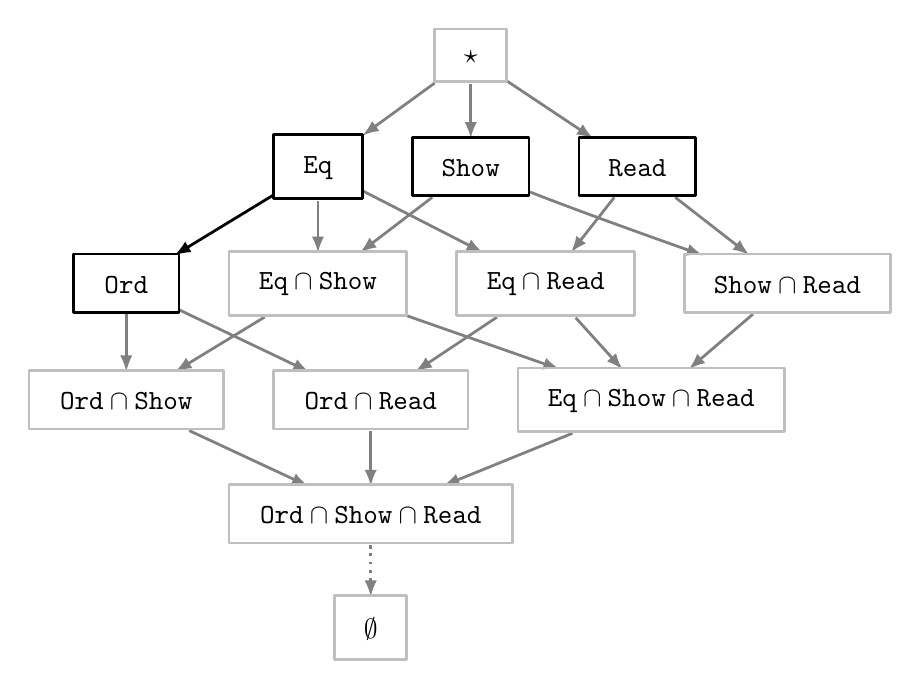
\begin{tikzpicture}[>=latex,line join=bevel,]
  \pgfsetlinewidth{1bp}
%%
\pgfsetcolor{black}
  % Edge: \texttt{Read} -> \texttt{Show} \cap \texttt{Read}
  \pgfsetcolor{gray}
  \draw [->] (232.63bp,167.4bp) .. controls (238.21bp,163.06bp) and (244.82bp,157.92bp)  .. (259.19bp,146.74bp);
  % Edge: \texttt{Eq} \cap \texttt{Read} -> \texttt{Eq} \cap \texttt{Show} \cap \texttt{Read}
  \draw [->] (196.79bp,124.08bp) .. controls (199.91bp,120.62bp) and (203.41bp,116.76bp)  .. (213.58bp,105.52bp);
  % Edge: \texttt{Eq} \cap \texttt{Show} \cap \texttt{Read} -> \texttt{Ord} \cap \texttt{Show} \cap \texttt{Read}
  \draw [->] (195.6bp,82.47bp) .. controls (184.09bp,77.798bp) and (170.67bp,72.351bp)  .. (149.12bp,63.601bp);
  % Edge: \texttt{Ord} \cap \texttt{Show} -> \texttt{Ord} \cap \texttt{Show} \cap \texttt{Read}
  \draw [->] (57.662bp,83.441bp) .. controls (67.824bp,78.707bp) and (79.99bp,73.039bp)  .. (100.41bp,63.523bp);
  % Edge: \texttt{Eq} -> \texttt{Eq} \cap \texttt{Read}
  \draw [->] (120.2bp,169.7bp) .. controls (129.92bp,164.72bp) and (142.63bp,158.22bp)  .. (163.31bp,147.62bp);
  % Edge: \texttt{Eq} \cap \texttt{Show} -> \texttt{Ord} \cap \texttt{Show}
  \draw [->] (84.78bp,124.3bp) .. controls (77.557bp,119.9bp) and (69.215bp,114.83bp)  .. (52.699bp,104.77bp);
  % Edge: \texttt{Eq} \cap \texttt{Read} -> \texttt{Ord} \cap \texttt{Read}
  \draw [->] (168.45bp,124.3bp) .. controls (162bp,120bp) and (154.57bp,115.05bp)  .. (139.16bp,104.77bp);
  % Edge: \texttt{Eq} -> \texttt{Ord}
  \pgfsetcolor{black}
  \draw [->] (87.997bp,168.26bp) .. controls (79.995bp,163.39bp) and (70.108bp,157.37bp)  .. (52.367bp,146.57bp);
  % Edge: \texttt{Ord} \cap \texttt{Show} \cap \texttt{Read} -> \emptyset
  \pgfsetcolor{gray}
  \draw [->,dotted] (123bp,42.228bp) .. controls (123bp,39.648bp) and (123bp,36.8bp)  .. (123bp,23.708bp);
  % Edge: \texttt{Show} \cap \texttt{Read} -> \texttt{Eq} \cap \texttt{Show} \cap \texttt{Read}
  \draw [->] (260.64bp,125.4bp) .. controls (256.02bp,121.45bp) and (250.64bp,116.83bp)  .. (237.57bp,105.63bp);
  % Edge: \kindStar -> \texttt{Read}
  \draw [->] (172.02bp,209.32bp) .. controls (178.56bp,204.96bp) and (186.7bp,199.53bp)  .. (203.01bp,188.66bp);
  % Edge: \texttt{Read} -> \texttt{Eq} \cap \texttt{Read}
  \draw [->] (210.67bp,167.4bp) .. controls (207.86bp,163.82bp) and (204.63bp,159.71bp)  .. (195.14bp,147.63bp);
  % Edge: \texttt{Show} -> \texttt{Eq} \cap \texttt{Show}
  \draw [->] (145.12bp,167.4bp) .. controls (139.7bp,163.26bp) and (133.32bp,158.39bp)  .. (119.23bp,147.63bp);
  % Edge: \kindStar -> \texttt{Show}
  \draw [->] (159bp,208.32bp) .. controls (159bp,205.45bp) and (159bp,202.19bp)  .. (159bp,188.72bp);
  % Edge: \kindStar -> \texttt{Eq}
  \draw [->] (145.97bp,208.52bp) .. controls (140.64bp,204.65bp) and (134.3bp,200.03bp)  .. (120.09bp,189.7bp);
  % Edge: \texttt{Show} -> \texttt{Show} \cap \texttt{Read}
  \draw [->] (180.27bp,169.38bp) .. controls (183.19bp,168.23bp) and (186.17bp,167.07bp)  .. (189bp,166bp) .. controls (203.22bp,160.62bp) and (218.88bp,154.95bp)  .. (242.57bp,146.56bp);
  % Edge: \texttt{Ord} -> \texttt{Ord} \cap \texttt{Show}
  \draw [->] (35bp,125.4bp) .. controls (35bp,122.14bp) and (35bp,118.44bp)  .. (35bp,104.74bp);
  % Edge: \texttt{Eq} \cap \texttt{Show} -> \texttt{Eq} \cap \texttt{Show} \cap \texttt{Read}
  \draw [->] (136.16bp,124.74bp) .. controls (150.05bp,119.88bp) and (166.51bp,114.12bp)  .. (190.92bp,105.58bp);
  % Edge: \texttt{Eq} -> \texttt{Eq} \cap \texttt{Show}
  \draw [->] (104bp,166.08bp) .. controls (104bp,163.44bp) and (104bp,160.57bp)  .. (104bp,147.52bp);
  % Edge: \texttt{Ord} \cap \texttt{Read} -> \texttt{Ord} \cap \texttt{Show} \cap \texttt{Read}
  \draw [->] (123bp,83.228bp) .. controls (123bp,80.286bp) and (123bp,76.996bp)  .. (123bp,63.559bp);
  % Edge: \texttt{Ord} -> \texttt{Ord} \cap \texttt{Read}
  \draw [->] (54.095bp,126.89bp) .. controls (65.051bp,121.66bp) and (79.08bp,114.96bp)  .. (100.84bp,104.58bp);
  % Node: \texttt{Show}
\begin{scope}
  \definecolor{strokecol}{rgb}{0.0,0.0,0.0};
  \pgfsetstrokecolor{strokecol}
  \draw (180bp,189bp) -- (138bp,189bp) -- (138bp,168bp) -- (180bp,168bp) -- cycle;
  \draw (159bp,178bp) node {$\texttt{Show}$};
\end{scope}
  % Node: \texttt{Ord}
\begin{scope}
  \definecolor{strokecol}{rgb}{0.0,0.0,0.0};
  \pgfsetstrokecolor{strokecol}
  \draw (54bp,147bp) -- (16bp,147bp) -- (16bp,126bp) -- (54bp,126bp) -- cycle;
  \draw (35bp,136bp) node {$\texttt{Ord}$};
\end{scope}
  % Node: \texttt{Eq} \cap \texttt{Show} \cap \texttt{Read}
\begin{scope}
  \definecolor{strokecol}{rgb}{0.75,0.75,0.75};
  \pgfsetstrokecolor{strokecol}
  \draw (272bp,106bp) -- (176bp,106bp) -- (176bp,83bp) -- (272bp,83bp) -- cycle;
  \definecolor{strokecol}{rgb}{0.0,0.0,0.0};
  \pgfsetstrokecolor{strokecol}
  \draw (224bp,94bp) node {$\texttt{Eq} \cap \texttt{Show} \cap \texttt{Read}$};
\end{scope}
  % Node: \texttt{Show} \cap \texttt{Read}
\begin{scope}
  \definecolor{strokecol}{rgb}{0.75,0.75,0.75};
  \pgfsetstrokecolor{strokecol}
  \draw (310bp,147bp) -- (236bp,147bp) -- (236bp,126bp) -- (310bp,126bp) -- cycle;
  \definecolor{strokecol}{rgb}{0.0,0.0,0.0};
  \pgfsetstrokecolor{strokecol}
  \draw (273bp,136bp) node {$\texttt{Show} \cap \texttt{Read}$};
\end{scope}
  % Node: \kindStar
\begin{scope}
  \definecolor{strokecol}{rgb}{0.75,0.75,0.75};
  \pgfsetstrokecolor{strokecol}
  \draw (172bp,228bp) -- (146bp,228bp) -- (146bp,209bp) -- (172bp,209bp) -- cycle;
  \definecolor{strokecol}{rgb}{0.0,0.0,0.0};
  \pgfsetstrokecolor{strokecol}
  \draw (159bp,218bp) node {$\kindStar$};
\end{scope}
  % Node: \texttt{Ord} \cap \texttt{Read}
\begin{scope}
  \definecolor{strokecol}{rgb}{0.75,0.75,0.75};
  \pgfsetstrokecolor{strokecol}
  \draw (158bp,105bp) -- (88bp,105bp) -- (88bp,84bp) -- (158bp,84bp) -- cycle;
  \definecolor{strokecol}{rgb}{0.0,0.0,0.0};
  \pgfsetstrokecolor{strokecol}
  \draw (123bp,94bp) node {$\texttt{Ord} \cap \texttt{Read}$};
\end{scope}
  % Node: \texttt{Eq} \cap \texttt{Show}
\begin{scope}
  \definecolor{strokecol}{rgb}{0.75,0.75,0.75};
  \pgfsetstrokecolor{strokecol}
  \draw (136bp,148bp) -- (72bp,148bp) -- (72bp,125bp) -- (136bp,125bp) -- cycle;
  \definecolor{strokecol}{rgb}{0.0,0.0,0.0};
  \pgfsetstrokecolor{strokecol}
  \draw (104bp,136bp) node {$\texttt{Eq} \cap \texttt{Show}$};
\end{scope}
  % Node: \texttt{Eq}
\begin{scope}
  \definecolor{strokecol}{rgb}{0.0,0.0,0.0};
  \pgfsetstrokecolor{strokecol}
  \draw (120bp,190bp) -- (88bp,190bp) -- (88bp,167bp) -- (120bp,167bp) -- cycle;
  \draw (104bp,178bp) node {$\texttt{Eq}$};
\end{scope}
  % Node: \texttt{Eq} \cap \texttt{Read}
\begin{scope}
  \definecolor{strokecol}{rgb}{0.75,0.75,0.75};
  \pgfsetstrokecolor{strokecol}
  \draw (218bp,148bp) -- (154bp,148bp) -- (154bp,125bp) -- (218bp,125bp) -- cycle;
  \definecolor{strokecol}{rgb}{0.0,0.0,0.0};
  \pgfsetstrokecolor{strokecol}
  \draw (186bp,136bp) node {$\texttt{Eq} \cap \texttt{Read}$};
\end{scope}
  % Node: \texttt{Ord} \cap \texttt{Show} \cap \texttt{Read}
\begin{scope}
  \definecolor{strokecol}{rgb}{0.75,0.75,0.75};
  \pgfsetstrokecolor{strokecol}
  \draw (174bp,64bp) -- (72bp,64bp) -- (72bp,43bp) -- (174bp,43bp) -- cycle;
  \definecolor{strokecol}{rgb}{0.0,0.0,0.0};
  \pgfsetstrokecolor{strokecol}
  \draw (123bp,53bp) node {$\texttt{Ord} \cap \texttt{Show} \cap \texttt{Read}$};
\end{scope}
  % Node: \emptyset
\begin{scope}
  \definecolor{strokecol}{rgb}{0.75,0.75,0.75};
  \pgfsetstrokecolor{strokecol}
  \draw (136bp,24bp) -- (110bp,24bp) -- (110bp,1bp) -- (136bp,1bp) -- cycle;
  \definecolor{strokecol}{rgb}{0.0,0.0,0.0};
  \pgfsetstrokecolor{strokecol}
  \draw (123bp,12bp) node {$\emptyset$};
\end{scope}
  % Node: \texttt{Ord} \cap \texttt{Show}
\begin{scope}
  \definecolor{strokecol}{rgb}{0.75,0.75,0.75};
  \pgfsetstrokecolor{strokecol}
  \draw (70bp,105bp) -- (0bp,105bp) -- (0bp,84bp) -- (70bp,84bp) -- cycle;
  \definecolor{strokecol}{rgb}{0.0,0.0,0.0};
  \pgfsetstrokecolor{strokecol}
  \draw (35bp,94bp) node {$\texttt{Ord} \cap \texttt{Show}$};
\end{scope}
  % Node: \texttt{Read}
\begin{scope}
  \definecolor{strokecol}{rgb}{0.0,0.0,0.0};
  \pgfsetstrokecolor{strokecol}
  \draw (240bp,189bp) -- (198bp,189bp) -- (198bp,168bp) -- (240bp,168bp) -- cycle;
  \draw (219bp,178bp) node {$\texttt{Read}$};
\end{scope}
%
\end{tikzpicture}

 }
	\caption{Alternative view for some \(\kindStar\) classes}
\end{figure}

\noindent
\begin{figure}
	\centering
	\scalebox{1.0}{ 
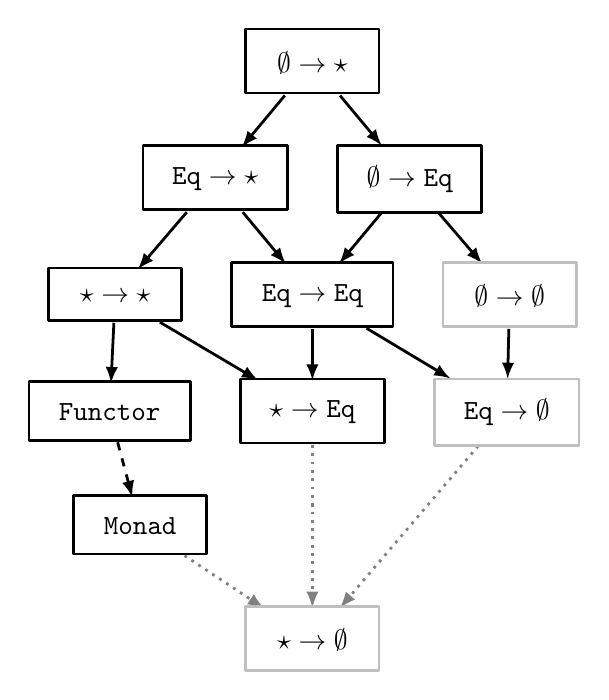
\begin{tikzpicture}[>=latex,line join=bevel,]
  \pgfsetlinewidth{1bp}
%%
\pgfsetcolor{black}
  % Edge: \kindStar \to \kindStar -> \kindStar \to \texttt{Eq}
  \draw [->] (47.111bp,126.47bp) .. controls (54.966bp,121.82bp) and (64.649bp,116.09bp)  .. (82.411bp,105.59bp);
  % Edge: \emptyset \to \texttt{Eq} -> \emptyset \to \emptyset
  \draw [->] (147.61bp,165.63bp) .. controls (150.36bp,162.41bp) and (153.39bp,158.88bp)  .. (163.09bp,147.57bp);
  % Edge: \texttt{Eq} \to \texttt{Eq} -> \texttt{Eq} \to \emptyset
  \draw [->] (121.5bp,124.3bp) .. controls (128.1bp,120.34bp) and (135.62bp,115.83bp)  .. (151.63bp,106.22bp);
  % Edge: \emptyset \to \texttt{Eq} -> \texttt{Eq} \to \texttt{Eq}
  \draw [->] (126.69bp,165.63bp) .. controls (124.01bp,162.41bp) and (121.06bp,158.88bp)  .. (111.64bp,147.57bp);
  % Edge: \emptyset \to \kindStar -> \emptyset \to \texttt{Eq}
  \draw [->] (111.94bp,208.08bp) .. controls (114.57bp,204.91bp) and (117.49bp,201.41bp)  .. (126.92bp,190.1bp);
  % Edge: \texttt{Eq} \to \texttt{Eq} -> \kindStar \to \texttt{Eq}
  \draw [->] (102bp,124.08bp) .. controls (102bp,121.44bp) and (102bp,118.57bp)  .. (102bp,105.52bp);
  % Edge: \emptyset \to \kindStar -> \texttt{Eq} \to \kindStar
  \draw [->] (92.064bp,208.08bp) .. controls (89.26bp,204.71bp) and (86.135bp,200.96bp)  .. (76.599bp,189.52bp);
  % Edge: \texttt{\texttt{Monad}} -> \kindStar \to \emptyset
  \pgfsetcolor{gray}
  \draw [->,dotted] (55.967bp,42.441bp) .. controls (62.122bp,38.371bp) and (69.321bp,33.61bp)  .. (84.562bp,23.532bp);
  % Edge: \texttt{Eq} \to \kindStar -> \texttt{Eq} \to \texttt{Eq}
  \pgfsetcolor{black}
  \draw [->] (76.936bp,166.08bp) .. controls (79.74bp,162.71bp) and (82.865bp,158.96bp)  .. (92.401bp,147.52bp);
  % Edge: \texttt{Eq} \to \emptyset -> \kindStar \to \emptyset
  \pgfsetcolor{gray}
  \draw [->,dotted] (161.67bp,81.901bp) .. controls (150.38bp,68.669bp) and (132.11bp,47.267bp)  .. (111.92bp,23.618bp);
  % Edge: \texttt{Eq} \to \kindStar -> \kindStar \to \kindStar
  \pgfsetcolor{black}
  \draw [->] (56.78bp,166.08bp) .. controls (53.385bp,162.12bp) and (49.533bp,157.62bp)  .. (39.189bp,145.55bp);
  % Edge: \kindStar \to \kindStar -> \texttt{\texttt{Functor}}
  \draw [->] (30.536bp,126.26bp) .. controls (30.372bp,122.81bp) and (30.18bp,118.78bp)  .. (29.503bp,104.57bp);
  % Edge: \texttt{\texttt{Functor}} -> \texttt{\texttt{Monad}}
  \draw [->,dashed] (31.89bp,83.228bp) .. controls (32.705bp,80.191bp) and (33.619bp,76.783bp)  .. (37.167bp,63.559bp);
  % Edge: \kindStar \to \texttt{Eq} -> \kindStar \to \emptyset
  \pgfsetcolor{gray}
  \draw [->,dotted] (102bp,82.251bp) .. controls (102bp,69.708bp) and (102bp,49.542bp)  .. (102bp,23.727bp);
  % Edge: \emptyset \to \emptyset -> \texttt{Eq} \to \emptyset
  \pgfsetcolor{black}
  \draw [->] (172.72bp,124.08bp) .. controls (172.66bp,121.62bp) and (172.59bp,118.95bp)  .. (172.29bp,106.1bp);
  % Node: \emptyset \to \texttt{Eq}
\begin{scope}
  \definecolor{strokecol}{rgb}{0.0,0.0,0.0};
  \pgfsetstrokecolor{strokecol}
  \draw (163bp,190bp) -- (111bp,190bp) -- (111bp,166bp) -- (163bp,166bp) -- cycle;
  \draw (137bp,178bp) node {$\emptyset \to \texttt{Eq}$};
\end{scope}
  % Node: \texttt{\texttt{Monad}}
\begin{scope}
  \definecolor{strokecol}{rgb}{0.0,0.0,0.0};
  \pgfsetstrokecolor{strokecol}
  \draw (64bp,64bp) -- (16bp,64bp) -- (16bp,43bp) -- (64bp,43bp) -- cycle;
  \draw (40bp,53bp) node {$\texttt{\texttt{Monad}}$};
\end{scope}
  % Node: \kindStar \to \texttt{Eq}
\begin{scope}
  \definecolor{strokecol}{rgb}{0.0,0.0,0.0};
  \pgfsetstrokecolor{strokecol}
  \draw (128bp,106bp) -- (76bp,106bp) -- (76bp,83bp) -- (128bp,83bp) -- cycle;
  \draw (102bp,94bp) node {$\kindStar \to \texttt{Eq}$};
\end{scope}
  % Node: \texttt{Eq} \to \kindStar
\begin{scope}
  \definecolor{strokecol}{rgb}{0.0,0.0,0.0};
  \pgfsetstrokecolor{strokecol}
  \draw (93bp,190bp) -- (41bp,190bp) -- (41bp,167bp) -- (93bp,167bp) -- cycle;
  \draw (67bp,178bp) node {$\texttt{Eq} \to \kindStar$};
\end{scope}
  % Node: \emptyset \to \kindStar
\begin{scope}
  \definecolor{strokecol}{rgb}{0.0,0.0,0.0};
  \pgfsetstrokecolor{strokecol}
  \draw (126bp,232bp) -- (78bp,232bp) -- (78bp,209bp) -- (126bp,209bp) -- cycle;
  \draw (102bp,220bp) node {$\emptyset \to \kindStar$};
\end{scope}
  % Node: \kindStar \to \kindStar
\begin{scope}
  \definecolor{strokecol}{rgb}{0.0,0.0,0.0};
  \pgfsetstrokecolor{strokecol}
  \draw (55bp,146bp) -- (7bp,146bp) -- (7bp,127bp) -- (55bp,127bp) -- cycle;
  \draw (31bp,136bp) node {$\kindStar \to \kindStar$};
\end{scope}
  % Node: \texttt{Eq} \to \texttt{Eq}
\begin{scope}
  \definecolor{strokecol}{rgb}{0.0,0.0,0.0};
  \pgfsetstrokecolor{strokecol}
  \draw (131bp,148bp) -- (73bp,148bp) -- (73bp,125bp) -- (131bp,125bp) -- cycle;
  \draw (102bp,136bp) node {$\texttt{Eq} \to \texttt{Eq}$};
\end{scope}
  % Node: \texttt{\texttt{Functor}}
\begin{scope}
  \definecolor{strokecol}{rgb}{0.0,0.0,0.0};
  \pgfsetstrokecolor{strokecol}
  \draw (58bp,105bp) -- (0bp,105bp) -- (0bp,84bp) -- (58bp,84bp) -- cycle;
  \draw (29bp,94bp) node {$\texttt{\texttt{Functor}}$};
\end{scope}
  % Node: \kindStar \to \emptyset
\begin{scope}
  \definecolor{strokecol}{rgb}{0.75,0.75,0.75};
  \pgfsetstrokecolor{strokecol}
  \draw (126bp,24bp) -- (78bp,24bp) -- (78bp,1bp) -- (126bp,1bp) -- cycle;
  \definecolor{strokecol}{rgb}{0.0,0.0,0.0};
  \pgfsetstrokecolor{strokecol}
  \draw (102bp,12bp) node {$\kindStar \to \emptyset$};
\end{scope}
  % Node: \texttt{Eq} \to \emptyset
\begin{scope}
  \definecolor{strokecol}{rgb}{0.75,0.75,0.75};
  \pgfsetstrokecolor{strokecol}
  \draw (198bp,106bp) -- (146bp,106bp) -- (146bp,82bp) -- (198bp,82bp) -- cycle;
  \definecolor{strokecol}{rgb}{0.0,0.0,0.0};
  \pgfsetstrokecolor{strokecol}
  \draw (172bp,94bp) node {$\texttt{Eq} \to \emptyset$};
\end{scope}
  % Node: \emptyset \to \emptyset
\begin{scope}
  \definecolor{strokecol}{rgb}{0.75,0.75,0.75};
  \pgfsetstrokecolor{strokecol}
  \draw (197bp,148bp) -- (149bp,148bp) -- (149bp,125bp) -- (197bp,125bp) -- cycle;
  \definecolor{strokecol}{rgb}{0.0,0.0,0.0};
  \pgfsetstrokecolor{strokecol}
  \draw (173bp,136bp) node {$\emptyset \to \emptyset$};
\end{scope}
%
\end{tikzpicture}

 }
	\caption{Some \(\emptyset \to \kindStar\) classes}
\end{figure}

\begin{example}~
\[ \texttt{id} :: \forall a \in {\kindStar} \, . \, a \to a \]
\[ \texttt{const} :: \forall a \in {\kindStar} \, . \, \forall b \in {\kindStar} \, . \, a \to b \to a \]
\end{example}

\begin{example}~
\[ \texttt{1} :: \forall a \in \texttt {Num} \, . \, a \]
\[ \texttt{elem} :: \forall a \in \texttt{Eq} \, . \, a \to [a] \to \texttt{Bool} \]
\end{example}

\begin{example}~
\begin{code}
ex :: (C1 a,C2 a) => a
\end{code}
\[ \texttt{ex} :: \forall \, a \in \texttt{C1} \cap \texttt{C2} \, . \, a \]
\end{example}

\begin{example}
This one is ugly and points out some problems.
\begin{code}
ex :: (Eq (m a), Monad m) => m a -> a -> Bool
ex x y = x == return y
\end{code}
There are few possibilities how to deal with this. For example
\[ \texttt{ex} :: \forall m \in \texttt{Monad} \cap \emptyset \to \texttt{Eq} \, . \, \forall m \, a \in \texttt{Eq} \, . \, m \, a \to a \to \texttt{Bool} \]
but this would require to make possible quantification not only over variables but over applications too.
% We will rather stick with following alternative:
Alternatively, taking \(\{\_\}\) as a meta-operator mapping type to singleton kind,
it is possible to express desired type by
\[ \texttt{ex} :: \forall a \in \kindStar \, . \, \forall m \in \texttt{Monad} \cap \{ a \} \to \texttt{Eq} \, . \, m \, a \to a \to \texttt{Bool} \]
Both mentioned possibilities embodies some ``dependency'', that gives significance to order of quantifications.
We will show how to deal with this later. % XXX : later... multiparam type classes.
\end{example}

\begin{example}~
\begin{code}
ex :: (Monad m, Eq (m a), Eq a) => m a -> a -> Bool
ex x y = y == y && x == return y
\end{code}
\[ \texttt{ex} :: \forall m \in \texttt{Monad} \cap (\texttt{Eq} \to \texttt{Eq}) \, . \, \forall a \in \texttt{Eq} \, . \, m a \to a \to \texttt{Bool} \]
\end{example}

This leads to situation, where one th

Contexts, context reductions... blah blah... much better solution -- watch this:
\begin{align*}
	\tau   & ::= \forall \, a \in \kappa \, . \, \tau ~|~ \sigma \\
	\sigma & ::= a ~|~ \sigma \to \sigma ~|~ \rho \, \sigma \\
	\rho   & ::= a ~|~ \rho \, \sigma \\
	\kappa & ::= c ~|~ \kindStar ~|~ \kappa \to \kappa ~|~ \kappa \cap \kappa \\
\end{align*}
where
\begin{itemize}
	\item \(a\) stands for type variable,
	\item \(c\) stands for kind constant,
	\item \(\tau\) represents types,
	\item and \(\kappa\) represents kinds.
\end{itemize}

Key in understanding this fact (noticed by \cite{libor}),
that as classes are sets of type constructors, they are kinds.
Not only that, they form obvious structure~-- intersection-semilattice.

Type class declaration creates new kind constant.
Instances fill selected classes (constants explicitly, others implicitly).
Analogously \texttt{data} creates and fills types.

% XXX: Is it really sort that matters?
Intersection have sense (understand possibility of not-emptiness) only on
kinds with same sort(?) (\(\texttt{Eq} \cap \texttt{Functor}\) even feels wrong).

Inclusion diagrams accompanying some distinguished type classes can be found for
example in \cite{typeclassopedia}.

% XXX: Eventually remove this text and if possible replace
%      with 15 pages of text ;-).
This was expected to generate like 15 pages in thesis \verb~:-/~.

\section{Removing type-class infrastructure}

As noticed by many and underlined by actual implementation, type-classes can be removed
from the language with only little ``harm''.

Let us have a look at how it can be done. Take the following well known example.
\begin{code}
class Eq a where
    (==), (/=) :: a -> a -> Bool
\end{code}
And definitions that employ this class.
\begin{code}
(==) :: Eq a => a -> a -> Bool
elem :: Eq a => a -> [a] -> Bool
elem = any . (==)
f :: Eq a => a -> [[a]] -> Bool
f = any . elem
\end{code}
This can be expressed in following way:
\begin{code}
type Eq a = (a -> a -> Bool,a -> a -> Bool)
\end{code}
with definitions
\begin{code}
(==) :: Eq a -> a -> a -> Bool
(==) = fst

elem :: Eq a -> a -> [a] -> Bool
-- elem ((==),(/=)) = any . (==)
-- or
elem i = any . (==) i

f :: Eq a -> a -> [[a]] -> Bool
f i = any . elem i
\end{code}

One may naturally wonder, how it would be with non-\(\kindStar\) classes.
Take \texttt{Monad}.
\begin{code}
class Monad m where
	return :: a -> m a
	(>>=) :: m a -> (a -> m b) -> m b
\end{code}
(Function \texttt{fail} is omitted intentionally but can be added with
no problem.)
Most straightforward way how to express it would be
\begin{code}
type Monad m a b = (a -> m a,m a -> (a -> m b) -> m b)
\end{code}
But what have we done? This is not traditional \texttt{Monad} but
multi-parameter. This is another example for multi-parameter type classes
being natural. But how to do it intended way?
\begin{code}
type Monad m = forall a b . (a -> m a,m a -> (a -> m b) -> m b)
\end{code}


\chapter{Extensions}

This chapters goes trough various type extensions showing examples
what can be achieved using them with focus on what they have in common
and where they differ.

\section{Empty data declarations}

% This extension is implemented in \texttt{GHC} and can be enabled via
% \texttt{LANGUAGE} pragma \texttt{EmptyDataDecls}.
The extension described in this paragraph was included in Haskell 2010 standard.

Extension \emph{empty data declarations} allows empty data declarations
(without any data constructors). This is very natural as there is possible
to declare types with arbitrary number of constructors (except 0). In
fact, it is not extension in sense of adding something artificial in
language, it only make syntax more comprehensive. Using this extension can
be empty (except \(\bot\)) data type \texttt{Empty} declared in this way:
\begin{code}
data Empty
\end{code}
However, the same can be achieved without this extension as well. Consider type \texttt{Empty'}
declared with \texttt{newtype}.
\begin{code}
newtype Empty' = E' Empty'
\end{code}
It looks like there actually are values besides \(\bot\), namely \(\texttt{E'}^n \, \bot\)
for every \(n \in \mathbb{N}_0\) and \(\mu x . \texttt{E'} \, x\).
Those are, as shown in lemma \ref{emptyTypes}, indistinguishable from \(\bot\).

\begin{lemma}[Empty types]
\label{emptyTypes}
If there is value \(v :: \texttt{Empty'}\), then \(v \approx \bot\).
\end{lemma}

\begin{proof}
In \cite{haskell2010} is stated, that \(\texttt{Empty'} \, \bot \approx \bot\).
Simple induction provides us all \(\texttt{E'}^n \, \bot\) cases
and least fixed point case is obvious as well, as \(\bot\) is least element.
\end{proof}

This ``extension'' is in fact very natural. Definition of \texttt{Empty'}
might give user feeling that it is non-empty, whereas emptiness is
obvious in case of \texttt{Empty}.

Analogous construction can be done with type constructors.

When defining empty type without this extension be sure to use
\texttt{newtype}, not \texttt{data}, as it will be inhabited not only with \(\bot\).
\begin{code}
data EmptyBad = EB EmptyBad
\end{code}

\begin{lemma}
There exists value \(v :: \texttt{EmptyBad}\) such that \(v \not \approx \bot\).
\end{lemma}

\begin{proof}
Let \texttt{emptyBad} be catamorphism over \texttt{EmptyBad}.
\begin{code}
emptyBad :: (a -> a) -> EmptyBad -> a
emptyBad f (EB x) = f (emptyBad x)
\end{code}
Now consider \(\texttt{emptyBad fac (fix EB)}\) and \(\texttt{emptyBad fac} \, \bot\).
They are obviously distinguishable as first one is factorial function but second one is \(\bot\) itself.
\end{proof}

\section{Multi-parameter type classes}

This extension is implemented in \texttt{GHC} and can be enabled via
\texttt{LANGUAGE} pragma \texttt{MultiParamTypeClasses}.

\subsection{Functional dependencies}

\subsection{Relaxed rules for instances}

\subsubsection{Relaxed rules for the instance head}

\texttt{TypeSynonymInstances} Not much interesting.

\subsubsection{Relaxed rules for instance contexts}

\begin{itemize}
\item \texttt{FlexibleContexts}
\item \texttt{UndecidableInstances}
\item \texttt{OverlappingInstances} \texttt{IncoherentInstances}
\end{itemize}

\subsection{Examples}

Subtyping.

\section{Generalised algebraic datatypes}

\section{Extensible kinds}

\section{Rank-2 types}

\subsection{Rank-n types}

% \section{Subtyping} % as example

\chapter{Examples}

\section{Apples and oranges}

Problem is simple: we do not want do jumble apples and oranges,
exactly like we were taught in elementary school.

\subsection{Type synonyms}

Simplest way how to ``differentiate'' fruit under discussion is to define
appropriate type synonyms.
\begin{code}
type Apples  = Integer
type Oranges = Integer
\end{code}
These alternative names can be now used in type signatures to signalise that
particular value represents amount of apples/oranges.

Advantages of this solution include possibility to use all power we have
to manipulate original type (\texttt{Integer} in this case). On the contrary,
safety requirement have not been met, as those type synonyms are equivalent
during type checking. Compiler will have no problem with
code like \texttt{(15 :: Apples) + (27 :: Oranges)}.

\subsection{Type Classes}

Type classes provide another possible solution. We define newtype wrapper
for each fruit type.
\begin{code}
newtype Apples  = Apples  Integer
newtype Oranges = Oranges Integer
\end{code}

Addition of two representations of same type of fruit is always semantically
the same, so we want to call it the same name. Overloading of this kind is what
type classes were introduced into the language.
\begin{code}
class Fruit a where
    plus :: a -> a -> a
instance Fruit Apples where
	Apples x `plus` Apples y = Apples (x + y)
instance Fruit Oranges where
	Oranges x `plus` Oranges y = Oranges (x + y)
\end{code}

\subsection{Phantom types \& Empty data declarations}

This solution is simple and clean.
\begin{code}
data Apple
data Orange

newtype Count a = Count Integer

plus :: Count a -> Count a -> Count a
Count x `plus` Count y = Count (x + y)
\end{code}
The most interesting thing here is function \texttt{plus}, that itself has a more general type, but
by narrowing it down to more specific one we get a function that allows us
adding up oranges with oranges, apples with apples, but forbids any other combinations
of apples and oranges. Advantage of this solution is that it is polymorphic
and we do not need to separately write code for apples and oranges.

On the contrary, this can be also seen as drawback, as one can create value
of type \texttt{Count Bool} which we have not intended. However,
one can take this in count by writing:
\begin{code}
data Apple
data Orange

class Fruit a where

instance Fruit Apple
instance Fruit Orange

newtype Count a = Count Integer

plus :: Fruit a => Count a -> Count a -> Count a
Count x `plus` Count y = Count (x + y)
\end{code}

As every elementary school child notices, from time to time one need to add apples and oranges,
and result will not be such nonsense:
\begin{code}
data Fruit'
instance Fruit Fruit'

plus' :: Fruit a => Count a -> Count b -> Count Fruit'
Count x `plus'` Count y = Count (x + y)
\end{code}

\chapter{Unified view}

% \chapter{Own extension proposal}

%\chapter{Z\'aver}
\chapter{Conclusion}

I came to conclusion that violet cows are present mainly in ads.

%\bibliographystyle{apalike}
\bibliographystyle{plain}
\bibliography{bibliography}

\end{document}
